\documentclass[conference]{IEEEtran}
\usepackage{graphicx}
\usepackage[utf8]{inputenc}
\usepackage[T1]{fontenc}
\usepackage[polutonikogreek,english]{babel}

\newcommand{\greek}[1]{{\selectlanguage{polutonikogreek}#1}}

\hyphenation{op-tical net-works semi-conduc-tor}

\begin{document}
\bstctlcite{IEEEexample:BSTcontrol}

\title{Model Predictive Control for\\Underwater Robots in Ocean Waves}

\author{\IEEEauthorblockN{Daniel Fernández}
\IEEEauthorblockA{School of Mechanical, Industrial\\and Manufacturing Engineering\\
Oregon State University\\
Corvallis, Oregon 97331--6001\\
Email: fernanda@oregonstate.edu}
\and
\IEEEauthorblockN{Geoffrey Hollinger}
\IEEEauthorblockA{School of Mechanical, Industrial\\and Manufacturing Engineering\\
Oregon State University\\
Corvallis, Oregon 97331--6001\\
Email: geoff.hollinger@oregonstate.edu}
}

% make the title area
\maketitle


\begin{abstract}
%\boldmath
Autonomous marine vehicle decision making is an active avenue of research in the Field Robotics Community. Much of this work includes advancing underwater path planning, localization, and perception. Developments in this field can lead to cost-effective methods of deploying marine energy arrays. The purpose of this document is to summarize some of the more promising research applications as well as justify the use of autonomy in the offshore community.  
\end{abstract}

\begin{IEEEkeywords}	
marine robotics, wave energy, autonomous path planning, perception, oceanographic monitoring, SLAM, AUV, ROV
\end{IEEEkeywords}

\section{Introduction} 
\label{sec:introduction}

This paper is organized into the following sections. First, the remainder of section \ref{sec:intro} contains a brief intro to wave energy extraction and marine vehicles. Section \ref{sec:related} is divided into four subsections detailing relevant research in vehicle path planning, localization, perception, and combined applications. Concluding Remarks are then provided. Figure \ref{fig:structure} shows the paper outline in more detail. 

\subsection{Wave Energy}
The world's oceans can produce close to 2 TW -- roughly twice the current global usage -- of usable wave energy \cite{falnes}. Compared to solar and wind sources, wave energy is relatively predictable and available on a constant basis. Some challenges facing wave energy extraction are: poor scaled economics, a high rate of infrastructure wear, and unclear effects to the coastal geomorphology. All of these are active areas of research in the field.

According to Linear Wave Theory (LWT), the energy in one water wavelength is the sum of its potential and kinetic energies \cite{D&D}. After some derivation it is reduced to: 
\begin{equation}
E_L = 1/8 \rho g H^2 L
\end{equation}
Though simplified, this relationship illustrates a noteworthy point that neither the average potential nor kinetic energy per unit area depends on water depth, but instead is simply proportional to the squared waveheight term, H. The rate at which energy is transferred is the energy flux, and for LWT it is the rate at which work is being done by change in energy density of a fluid over a vertical face \cite{D&D}.

\begin{figure*}
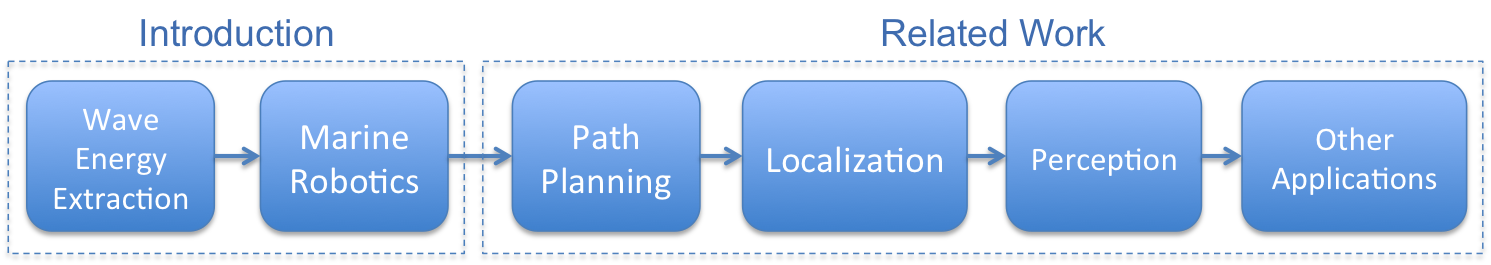
\includegraphics[width=\textwidth]{structure}
\caption{Section \ref{sec:intro} contains an introduction to wave energy conversion and marine vehicles. Section \ref{sec:related} is divided into four subsections detailing relevant research in 
vehicle path planning, perception, localization, and combined applications.}
\centering
\label{fig:structure}
\end{figure*}

Wave energy conversion as a whole is a young industry, and as such, as many competing converter designs. Point absorbers are small devices that freely oscillate at the water surface, expanding and contracting some working fluid. An attenuator is a jointed body that floats parallel to the wave direction, generating energy from the relative motion at the joint. An Oscillating Water Column (OWC) device uses differences in atmospheric pressure to force trapped air through a turbine as it is forced out by wave action \cite{falnes}. The arrays to be deployed at NNMREC test sites are yet to be determined; however, they will all require similar mooring and anchor systems. Thus, immediate robotic testing for ALFA is within reason.

\subsection{Marine Platforms}
Underwater vehicles can be classified into one of two generic categories: manned and unmanned vehicles. Unmanned Underwater Vehicles (UUV) are often labeled as synonymous with Autonomous Underwater Vehicles (AUV). This can be misleading as it is not an accepted standard. For the scope of this paper, the term AUV will be used for an untethered unmanned vehicle. The term Remotely Operated Vehicle (ROV) will be used to describe a tethered manned vehicle whose operation may or may not be tele-operated \cite{ROV}. No manned vehicles will be discussed.

The term ``glider'' may on occasion be used to describe a type of AUV. Gliders such as the Slocum shown in Figure \ref{fig:slocum} are designed to move efficiently through the water column by changing their weight \cite{bachmayer}. Successive pitch adjustments up and down result in a sawtooth profile with no external propulsion.

\begin{figure}[h]
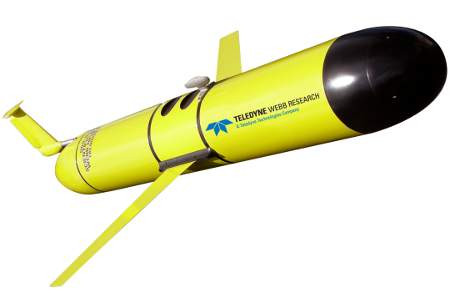
\includegraphics[width=0.95\columnwidth]{slocum}
\centering
\caption{A Webb Research Slocum Glider. This AUV uses only a buoyancy differential and small attitude adjustments to achieve an ultra low-wattage (0.5-1.0 Watts) and long range mission profile.}
\centering
\label{fig:slocum}
\end{figure}

\section{Model Predictive Control} \label{sec:related}

\section{System Dynamics} \label{sec:dynamics}

\section{Simulator} \label{sec:sim}

\section{Results} \label{sec:results}

\section{Conclusion} \label{sec:conclusion}
This paper presented some of the accomplishments in the marine robotic community. These included advancements in autonomous underwater path planning, localization, and perception. Efficient path planning helps reduce overall mission cost and time by optimizing methods of navigating. Localization issues in an environment absent GPS and long range wireless transmissivity prioritize the need for well-developed SLAM techniques with minimal input. Robotic perception in the underwater domain further complicates research efforts. In addition, multi-agent research such as the multi-glider work in \cite{leonard} is an excellent demonstration of the value of autonomy in performing oceanographic monitoring.

These advancements in underwater autonomy will be pivotal in the development of offshore energy arrays, since low-cost robotic platforms inspecting, monitoring, and manipulating infrastructure can reduce deployment costs drastically. Over the course of the NNMREC ALFA project, robust algorithms for these marine platforms to support WEC's will lead to improved scaled economics and further global wave energy development. As more challenges are addressed, this will help secure wave energy extraction as the premier sustainable energy source for the 21st century.


%\appendices
%\section{HERE WE GO}
% garbage

% use section* for acknowledgement

\section*{Acknowledgments}
This work is supported by Department of Energy Grant number DE-EE-0006816.0000.

\ifCLASSOPTIONcaptionsoff
  \newpage
\fi

% trigger a \newpage just before the given reference
% number - used to balance the columns on the last page
% adjust value as needed - may need to be readjusted if
% the document is modified later
%\IEEEtriggeratref{8}
% The "triggered" command can be changed if desired:
%\IEEEtriggercmd{\enlargethispage{-5in}}

\nocite{ballard, MAS}

\bibliography{main}
\bibliographystyle{IEEEtran}

%\end{main}

%\begin{thebibliography}{1}

%\bibitem{IEEEhowto:kopka}
%H.~Kopka and P.~W. Daly, \emph{A Guide to \LaTeX}, 3rd~ed.\hskip 1em plus
%  0.5em minus 0.4em\relax Harlow, England: Addison-Wesley, 1999.

%\end{thebibliography}

% biography section
% 
% If you have an EPS/PDF photo (graphicx package needed) extra braces are
% needed around the contents of the optional argument to biography to prevent
% the LaTeX parser from getting confused when it sees the complicated
% \includegraphics command within an optional argument. (You could create
% your own custom macro containing the \includegraphics command to make things
% simpler here.)
%\begin{biography}[{\includegraphics[width=1in,height=1.25in,clip,keepaspectratio]{mshell}}]{Michael Shell}
% or if you just want to reserve a space for a photo:

%\begin{IEEEbiography}[{\includegraphics[width=1in,height=1.25in,clip,keepaspectratio]{picture}}]{John Doe}
%\blindtext
%\end{IEEEbiography}

% You can push biographies down or up by placing
% a \vfill before or after them. The appropriate
% use of \vfill depends on what kind of text is
% on the last page and whether or not the columns
% are being equalized.

%\vfill

% Can be used to pull up biographies so that the bottom of the last one
% is flush with the other column.
%\enlargethispage{-5in}




% that's all folks
\end{document}
